\subsection{Neural Networks}
This section introduces the main concepts related to neural networks. Neural networks have been around since the 1940s and could initially handle only one hidden layer. But with the development of technologies and hardware it became possible to build deeper, more effective architectures, which leads to deep learning as we know it today. \par



\subsubsection{Brief History}


At first, neural networks were inspired by how the biological brain works, which is why deep learning was also called artificial neural networks (ANNs)\cite{Goodfellow-et-al-2016}. In biology, a neuron is the cell that receives, processes and transmits information to other neurons through connections called synapses \cite{neuron}. On the other hand, artificial neurons are defined as computational units (usually mathematical functions) that take one or more inputs and generate an output. \par

McCulloch and Pits designed an initial version of the neuron as a linear model in 1943, aiming to replicate brain function \cite{REF:11}:


\begin{equation}
f(x,w)=x1*w1 +x2*w2 +...+xn*wn
\end{equation}
where $x_1, ..., x_n$ are the input values and $w_1, ..., w_2$ is a set of hand-chosen weights.

\subsubsection{Components of an artificial neural network}

A simple artificial neural network (ANN) consists of input layer, hidden layer and output layer, where the values of the hidden layer are used as inputs for the output layer. A network with several layers is known as a deep neural network. Data flows through the neurons of the layer. Each neuron transforms the input it receives and sends it to the next layer. The neurons share the same characteristics regardless of the layer they are part of. \par



The Neuron, also called node, is the basic unit of a neural network. It's main components include inputs,
weights, activation function and output(s). From a high level point of view the inputs are multiplied by 
weights, then an activation function is applied to the result and finally, another function computes the output\cite{REF:12}\cite{REF:13}. \par


\begin{itemize}
	\item Weights are defined as adaptive coefficients, whose values are changed during the learning process. They represent the strength of the connection between units. A weight decides how much impact the input will have on the output.
	
	\item The summation function helps combine the input and weights, before passing the result to the activation function. Denote the input as $X = [x_1, x_2, ...x_n]$ and the weight vector as $W = [w_1, w_2, ...w_n]$.\\
	The summation function could be defined as the dot product between these two vectors:\\
	\begin{equation}
	X \cdot W =x_1 \cdot w_1 +x_2 \cdot w_2 +...+x_n \cdot w_n
	\end{equation}

	
	The summation function could instead compute the minimum, maximum etc. depending on the designated network architecture.The simplest form of an artificial neuron is a linear function which computes the weighted sum of inputs, to which, optionally, bias can be added:
	\begin{equation}
		y = \sum_{i=1}^{i=n}(x_i \cdot w_i) + b \textnormal{, where b is the bias, $x_i \in X, w_i \in W$}
	\end{equation}

	
	\item The activation function transforms the result of the summation function (usually) in a non-linear way. Typically, it has a squashing effect. It serves as a threshold. It divides the original space into two partitions. It's main purpose is to make the neural network non-linear. We denote the activation function as g.
	\begin{equation}
		y = g(\sum_{i=1}^{i=n}(x_i \cdot w_i) + b) \textnormal{, where b is the bias, $x_i \in X, w_i \in W$}
	\end{equation}

	
	\begin{figure}[h]
		\caption[Common activation functions]{Common activation functions.\\
			Source: http://prog3.com/sbdm/blog/cyh24/article/details/50593400 }
		\centering
		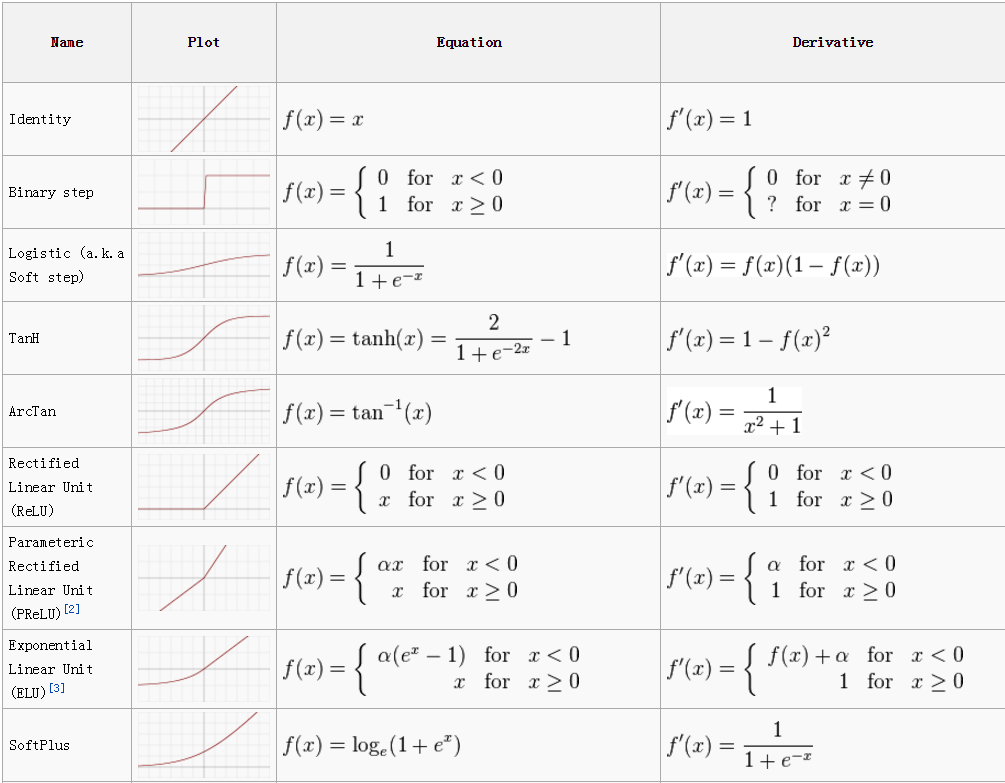
\includegraphics[width=1\textwidth, height=\textheight, keepaspectratio]{activation}
	\end{figure}
	\item The output is usually the result of an activation function.
	
\end{itemize}

\clearpage
\subsubsection{Underfitting and Overfitting}
%reformulat + surse noi

Neural networks are able to learn complicated non-linear functions to fit any training set. On the downside, this may lead to overfitting where the neural network learns the training data so well that it is unable to generalize on new, unseen data. This problem can especially occur on datasets with a small amount of data to learn from. \par

Underfitting, the counterpart of overfitting, happens when a machine learning model isn’t complex enough to accurately capture relationships between a dataset’s features and a target variable. An underfitted model results in problematic outcomes on new data, or data that it wasn’t trained on, and many times performs poorly even on training data. \par


\begin{figure}[h]
	\caption[Example of overfitting and underfitting]{Example of overfitting and underfitting
		\\ image source vitalflux.com}
	\centering
	\includegraphics[width=1\textwidth, height=\textheight, keepaspectratio]{"resources/overfitting"}
\end{figure}

\subsubsection{Convolutional Neural Networks}
\par
Convolutional Neural Networks (CNNs) are a class of Deep Neural Networks,
specialized in analyzing images. They were inspired by biological processes.
The connectivity pattern between neurons resembles the animal visual cortex.
\cite{cnn} \par

\begin{figure}[h]
	\centering
	\caption[Typical convolutional neural network architecture]{Typical CNN architecture
		\\ image source https://en.wikipedia.org/wiki/File:Typical\_cnn.png}
	\label{fig:cnn}
	\includegraphics[width=1.1\textwidth, height=1.5\textheight, keepaspectratio]{"resources/typical_cnn"}
\end{figure}

\par
A convolutional neural network consists of an input and an output layer, as well as multiple hidden layers. The hidden layers are typically convolutional layers, RELU layers, pooling layers, fully connected layers and normalization layers. \cite{cnn_git}

\begin{itemize}
	\item \textbf{Pooling} layers reduce the dimension of the data by combining the outputs of neuron clusters at one layer into a single neuron in the next layer. 
\end{itemize}


%vitalflux.com/ image source. overfitting.png
